\documentclass[11pt,a4paper]{article}
\usepackage[T1]{fontenc}
\usepackage[utf8]{inputenc}
\usepackage{lmodern}
\usepackage[margin=2.5cm]{geometry}
\usepackage{microtype}
\usepackage{booktabs}
\usepackage{tabularx}
\usepackage{array}
\usepackage{enumitem}
\usepackage{xcolor}
\usepackage{tikz}
\usetikzlibrary{arrows.meta,positioning,fit,backgrounds,calc}
\usepackage[font=small,labelfont=bf]{caption}
\usepackage[numbers,sort&compress]{natbib}
\usepackage[hidelinks]{hyperref}

\setlist{itemsep=2pt,topsep=4pt}
\newcolumntype{L}{>{\raggedright\arraybackslash}X}

\title{\textbf{Boundry: Model-Free Admission and Independently\\Verifiable Records for AI-Proposed Actions}}
\author{Ben Mueller\\[2pt]
\small Boundry, Australia\\
\small ORCID \href{https://orcid.org/0009-0004-0550-1485}{0009-0004-0550-1485} \quad
\href{mailto:verify@boundry.tech}{verify@boundry.tech}}
\date{\small Preprint, version 1.0 \quad October 2026}

\begin{document}
\maketitle

\begin{abstract}
\noindent As AI systems move from producing text to taking actions, the questions that matter change: what exactly was done, under which rule, what was refused and why, and whether someone independent can check the answers without trusting the operator. In the common \emph{prompt $\rightarrow$ model $\rightarrow$ action} arrangement, the model's output is the decision and the history is reconstructed afterwards from logs the operator controls. We describe Boundry, a system in which a model, a person or a program may only \emph{propose} an action in a small declared language. A deterministic kernel that contains no model admits or refuses each proposal against declared rules, executes an admitted proposal from the same sealed bytes that were checked, records refusals as first-class signed outcomes, and appends every step to a signed, hash-chained record. That record can be checked offline by an independent verifier that shares no code with the kernel. We present the design, a threat model, a worked example that readers can reproduce with a public verifier, and an evaluation on synthetic workloads: rebuild of state from the record, detection of single-byte alteration, agreement between independent verifier implementations, and byte-for-byte reproducibility across machines and platforms. The record layer runs in production in two financial applications, the full governing core is demonstrated end to end on a test bench, and authority-based policy gating and independent time-stamping are built or specified and staged for rollout. The contribution is not a new cryptographic primitive but a composition of established ones into a single model-free, fail-closed and independently checkable record of what an AI system was permitted to do and did.
\end{abstract}

\section{Introduction}

Much work on AI safety asks how to make a model behave: training, prompting, filtering and monitoring. These approaches matter, but they share a feature: the model's output remains, directly or through a thin tool layer, the decision to act. When a model only answers questions, a mistake is a wrong answer that can be ignored. When a model acts, by changing a record, moving money or operating a system, a mistake is an effect that has already happened.

This paper takes a complementary position. The harms most often feared from AI agents are harms of \emph{action}, and the safety of an action need not live inside the model. It can live in a small, deterministic component through which every action must pass, that the model cannot reach or persuade, and whose every decision is recorded in a form a stranger can check.

The pattern is old. Proof assistants in the LCF tradition~\citep{gordon1979lcf}, and modern systems such as Lean~\citep{demoura2021lean4}, let anyone propose a proof, a person, a search procedure or an AI model, and trust only a small kernel that checks each step against fixed rules. Security engineering has the related ideas of a reference monitor that mediates every access~\citep{anderson1972planning} and of fail-safe defaults~\citep{saltzer1975protection}. Boundry applies this pattern to \emph{actions} checked against \emph{rules declared by people}, and adds two properties that proofs do not need: the action is executed from the bytes that were checked, and every decision, including every refusal, is recorded in a tamper-evident chain that an independent implementation can verify offline.

\paragraph{Contributions.}
\begin{enumerate}
  \item An architecture in which AI-proposed actions pass through a model-free, deterministic, fail-closed admission step, and are executed from the sealed bytes that were admitted (Section~\ref{sec:design}).
  \item Refusal treated as a first-class, signed, recorded outcome, and a closed verdict vocabulary for verification that separates ``could not be checked'' and ``the checking instrument failed'' from ``the check failed'' (Section~\ref{sec:verdicts}).
  \item An explicit threat model stating what is trusted and what is not (Section~\ref{sec:threat}).
  \item A public, offline verifier and evaluation kit, so that several central claims can be tested by readers rather than taken on trust, together with an evaluation of rebuild, tamper detection, verifier independence and reproducibility (Sections~\ref{sec:example} and~\ref{sec:eval}).
\end{enumerate}

\paragraph{Status.} Boundry is being rolled out in stages, and we label each claim with its stage: \emph{in production} (running on real records), \emph{demonstrated} (end to end on a test bench with synthetic data), \emph{built} (implemented, awaiting enablement), or \emph{specified} (designed, with implementation under way). The signed, hash-chained record layer is in production in two Australian financial applications. The full governing core (admission, refusal and execution from sealed bytes) is demonstrated, with production deployment following once a suitable first product is selected. Admission by declared operations is demonstrated; gating by recorded authority is specified. Independent time-stamping of checkpoints is built and scheduled for enablement. Section~\ref{sec:roadmap} sets out the stages and the next steps, including independent evaluation.

\section{Threat model and trust assumptions}\label{sec:threat}

\paragraph{What Boundry is designed to resist.}
\begin{itemize}
  \item \textbf{An untrusted author.} The model (or person, or program) that writes a proposal may be mistaken, manipulated by injected content, or adversarial. Boundry assumes nothing about the author's intent.
  \item \textbf{Divergence between what was approved and what was done.} An action must not be executed from anything other than the bytes that were admitted.
  \item \textbf{Silent after-the-fact alteration.} A change to any recorded entry must be detectable by a party who did not produce it.
  \item \textbf{A verifier that inherits the producer's defects.} Verification should not depend on the producer's own code.
\end{itemize}

\paragraph{What is trusted.}
\begin{itemize}
  \item The kernel's code and the integrity of the host on which it runs at the time of execution.
  \item Custody of the signing keys, and the distribution of the corresponding verifying keys to readers. In the public kit the verifying key ships with the kit itself, so a reader must trust that the key is the operator's.
  \item The people who declare the rules. Boundry applies the rules it is given; it does not judge whether they are good.
  \item The edge connectors that carry out an admitted effect (writing a record, sending a message), to the extent that they faithfully apply the sealed bytes they are given.
\end{itemize}

\paragraph{Out of scope.} Actions that reach the world by a route that does not pass through the kernel; compromise of the host or keys; the truth of inputs (Boundry checks that a declared process was followed, not that its inputs were correct); availability and denial of service; and side channels.

\paragraph{External anchoring.} The record is tamper-\emph{evident}: an edit is not prevented, but it cannot pass unnoticed. Because a single operator holds the signing key in current deployments, an external witness is what rules out an operator rewriting and re-signing a whole chain. Boundry provides this by anchoring signed checkpoints with an RFC~3161 time-stamping authority~\citep{rfc3161}, with a transparency log~\citep{rfc9162} as an alternative. The mechanism is built and is scheduled to be enabled on production checkpoints; from that point, the absence of rewriting becomes independently checkable rather than resting on the operator.

\section{Design}\label{sec:design}

\subsection{Three parts and one boundary}

Boundry separates three roles (Figure~\ref{fig:arch}). The \emph{author}, typically a model, reads a request and writes a proposal. The \emph{kernel} decides whether the proposal may run, runs it, and records both. The \emph{edges} are ordinary connector code that produce real-world effects, driven only by admitted, sealed proposals. A fourth component, the \emph{verifier}, sits outside the system entirely and reads the record.

The kernel is ordinary, deterministic software. It contains no model and cannot reach one: the governed code path has no route by which a model can be loaded or called. ``No model in execution'' does not mean ``no code in execution''; it means the code that decides and records contains no model.

\begin{figure}[t]
\centering
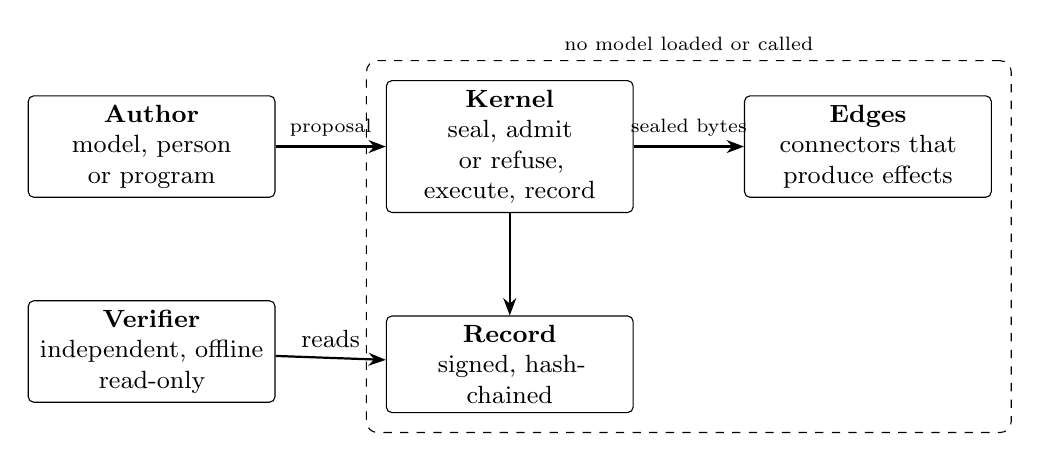
\begin{tikzpicture}[
  font=\small,
  box/.style={draw, rounded corners=2pt, align=center, minimum height=1.0cm, text width=2.9cm, fill=white},
  arr/.style={-{Stealth[length=2.2mm]}, thick},
  zone/.style={draw, dashed, rounded corners=4pt, inner sep=7pt}
]
\node[box] (author) {\textbf{Author}\\model, person\\or program};
\node[box, right=1.4cm of author] (kernel) {\textbf{Kernel}\\seal, admit or refuse,\\execute, record};
\node[box, right=1.4cm of kernel] (edges) {\textbf{Edges}\\connectors that\\produce effects};
\node[box, below=1.3cm of kernel] (record) {\textbf{Record}\\signed, hash-chained};
\node[box, below=1.3cm of author] (verifier) {\textbf{Verifier}\\independent, offline\\read-only};

\draw[arr] (author) -- node[above,font=\scriptsize]{proposal} (kernel);
\draw[arr] (kernel) -- node[above,font=\scriptsize]{sealed bytes} (edges);
\draw[arr] (kernel) -- (record);
\draw[arr] (verifier) -- node[above]{reads} (record);

\begin{scope}[on background layer]
\node[zone, fit=(kernel)(edges)(record), label={[font=\scriptsize]above:no model loaded or called}] {};
\end{scope}
\end{tikzpicture}
\caption{The author may only propose. The kernel is the only component that can authorise an effect; edges act only on admitted, sealed bytes. The verifier shares no code with the kernel and needs only the record and a verifying key.}
\label{fig:arch}
\end{figure}

\subsection{The life of a request}

\paragraph{Proposal.} The author expresses an intended action in a small declared language: which operation, on what, under whose authority. Requests in this language are finite, bounded, loop-free plans composed from a registered set of operations (\emph{primitives}). The language is deliberately not general-purpose. A proposal is only a suggestion; nothing has happened.

\paragraph{Seal.} The proposal is reduced to a canonical byte form, fingerprinted, signed, and bound to the requester and time. From this point it cannot be changed without detection.

\paragraph{Admit or refuse.} The kernel checks the sealed proposal against fixed rules: that it is a known, well-formed kind and that only permitted primitives appear. Anything not declared is refused. Reads and writes are scoped to a declared tenant, and a request with no declared scope is refused rather than widened. Admission extends to gating actions by recorded authority, with a verdict recorded before the effect; this stage is specified and its evaluation will follow implementation. Admission does not consult the author's reasoning, so injected text can change what is \emph{proposed} but cannot make a proposal pass that the declared rules do not permit. This follows from the architecture; testing it against an adversarial prompt-injection benchmark is a planned next step.

\paragraph{Execute from the sealed bytes.} An admitted proposal runs inside declared time, memory and work limits. Where an effect is produced at an edge, the edge is driven from the sealed proposal, never from the author's live output, so what was checked and what was done are the same bytes. On the bench, execution reads the sealed proposal and the record binds proposal, decision and result; edge connectors for external effects follow with the first production deployment of the core.

\paragraph{Record.} Every stage is sealed and appended to a chain in which each entry commits to the digest of its predecessor~\citep{schneier1999audit,crosby2009tamper}. Periodically the kernel signs a checkpoint over the record set, committing to its size and a Merkle-style root~\citep{merkle1987signature}. Checkpoint production is signalled from the append path at constant cost; deriving, signing and any external anchoring sit off that path, so an external party's outage cannot stall a seal.

\subsection{Properties of the construction}

\begin{itemize}
  \item \textbf{A canonical form that refuses ambiguity.} Two conforming implementations produce identical bytes for the same value. A value with two possible renderings is refused and named rather than approximated: floating-point numbers, keys that collide after Unicode normalisation, an absent field conflated with a null one. Numeric determinism comes from integers and fixed-point decimals. (Compare JCS~\citep{rfc8785}, which also rejects some values, such as non-finite numbers, but otherwise serialises numbers in a defined floating-point form.)
  \item \textbf{Identity independent of the signer.} What a record \emph{is} and who \emph{vouched for it} are separate. Identical work under different keys has one identity, and key rotation does not rewrite the past. Keys rotate by epoch; retiring a key is distinguished from revoking it.
  \item \textbf{Absence is explicit.} ``No predecessor'' is expressed by absence, not by a sentinel value that a reader might mistake for a real value or for failure. More generally, the design refuses and names an absent precondition rather than defaulting through it.
  \item \textbf{Content-addressed storage.} Record bodies are addressed by their hash, and an identifier cannot be rebound to different bytes.
  \item \textbf{Determinism as a measured property.} The runtime is declared, and undeclared non-deterministic dependencies are sought by perturbation rather than assumed absent. The cross-platform and clean-room results in Section~\ref{sec:eval} are the measurements we report.
\end{itemize}

\subsection{Refusal and the verdict vocabulary}\label{sec:verdicts}

A refusal is not an error, a retry or a silent default. It is a signed record with a stated reason, kept beside admissions. In the public evaluation kit, for example, a proposal that names a primitive outside the permitted set is refused at the resolution stage with the reason \texttt{primitive\_not\_in\_allowlist}, and that refusal is itself a verifiable record.

Verification uses a closed vocabulary (Table~\ref{tab:verdicts}). The \textsc{indeterminate} verdict is being finalised for the next verifier release. Comparison of two runs is reported separately, as \textsc{equivalent}, \textsc{divergent} or \textsc{unreachable}. Each verdict states both what it means and what it does not mean. Two distinctions matter most. First, \emph{absence of attestation is not falsity}: a record with nothing attesting to it is \textsc{unattested}, never ``false''. Second, \emph{failure of the instrument outranks any finding about the record}: if the verifier itself cannot complete, the result is \textsc{indeterminate} and says nothing about the record either way.

\begin{table}[t]
\centering\small
\caption{Verification verdicts, in order of precedence (highest first).}
\label{tab:verdicts}
\begin{tabularx}{\linewidth}{@{}lLL@{}}
\toprule
Verdict & Means & Does not mean \\
\midrule
\textsc{Indeterminate} & The verifier failed to complete. & Anything about the record. \\
\textsc{Altered} & A valid attestation exists and the content no longer matches it. & Who altered it, or when. \\
\textsc{Refuted} & Evidence was supplied and failed to verify. & Forgery or bad faith; corruption, a wrong key or truncation produce the same verdict. \\
\textsc{Unattested} & Nothing attests to these bytes. & That the record is false. \\
\textsc{Attested} & The named check ran and passed. & Anything beyond the stated scope. \\
\bottomrule
\end{tabularx}
\end{table}

\subsection{Independent verification}

The verifier, Boundry Verify~\citep{boundryverify}, is a separate, read-only package that runs on the reader's machine using only the Python standard library. It opens no socket, cannot sign, writes nothing, and attaches to no database; each of these properties is held by a named self-check with a planted control that the check must reject. It re-derives fingerprints, recomputes plan identities, walks each link from submitted intent to output, and compares runs by hash rather than by re-execution. Because it shares no code with the kernel, a defect in one is unlikely to be masked by the same defect in the other.

\section{A worked example readers can reproduce}\label{sec:example}

The public evaluation kit~\citep{boundryverify} contains real governed runs of the kernel on synthetic inputs: a calculation, a small transformation chain, and one refused request, each executed in fresh processes on macOS arm64 and on Linux aarch64. It also contains three deliberately tampered copies of one run (a forged hash, a changed output byte, a lost output) and one verifying key. Each run ships with its submitted intent beside it, because the record carries the intent's hash rather than the intent.

A reader with Python 3.12 or later can install the verifier and ask three questions:

\begin{enumerate}
  \item \emph{Compare the calculation run on macOS with the same run on Linux.} The result is \textsc{equivalent}. Outputs, plan body, result and payload signatures are byte-identical. The fields that differ are wall-clock stamps and hashes taken over them, together with descriptive metadata (the recorded environment and platform, and the run label); each is named and marked as expected.
  \item \emph{Compare the macOS run with its forged-hash copy.} The result is \textsc{divergent}: the forgery is caught by hash comparison, and the failing envelope is named.
  \item \emph{Explain the transformation run.} The verifier walks the lineage from submitted intent to output, recomputing each link offline.
\end{enumerate}

The refused run can be inspected in the same way: it is a signed record whose reason names the primitive that was not permitted. None of these steps requires access to the kernel or a network connection. They rely on the verifying key shipped with the kit. The kit demonstrates the refusal side of admission; a kit showing authority-based gating will follow that stage.

\section{Evaluation}\label{sec:eval}

Table~\ref{tab:eval} summarises what has been measured. Unless stated otherwise, results come from a test bench with synthetic data and freshly generated keys.

\begin{table}[t]
\centering\small
\caption{Evaluation summary. ``Bench'' means synthetic data on the developer's machines; ``kit'' means the public evaluation kit; ``production'' means live use on real records.}
\label{tab:eval}
\begin{tabularx}{\linewidth}{@{}>{\raggedright\arraybackslash}p{3.1cm}LL@{}}
\toprule
Property & Method & Result \\
\midrule
Test suites (bench) & Kernel suite; corpus gate; full programme test set on the primary machine & 2{,}199 passed, 0 failed; 283 passed; 3{,}603 passed, 6 skipped \\
Rebuild from record (bench) & 12 requests producing 144 sealed envelopes; state rebuilt from the record alone and compared & Identical; 144 form hashes re-derived; source unchanged \\
Tamper detection (bench) & One byte altered in a copy of a sealed record & Refused; altered body and both hashes named \\
Checkpoints (bench) & All checkpoints verified; heads recomputed from leaves; consecutive pairs checked for consistency; equivocation check & 144 of 144 verified and recomputed; of 143 consecutive pairs, 99 consistent and 44 at unchanged size (nothing to prove); 0 failures; no equivocation \\
Verifier independence (bench) & Kernel's own verifier vs.\ offline verifier on the same 144 bundles & Agree on 144 of 144; witness receipt \textsc{unattested} on all, as no witness exists \\
Second implementation (bench) & A separate Go verifier written from the specification, not ported, vs.\ the Python verifier & Agree on 148 of 148 vectors (internal; not published or third-party) \\
Clean-room rebuild (bench) & Second machine; only two sealed source bundles and an offline cache of 57 packages; network blocked & Source trees, commit identities and an engine digest over 175 files equal to the primary machine's published figures \\
Cross-platform determinism (kit) & Same governed requests on macOS arm64 and Linux aarch64, by different people & Byte-identical except wall-clock stamps, hashes over them, and descriptive run metadata \\
Rebuild throughput (bench) & Rebuild from empty, one machine & 100{,}000 records in 9.27\,s \\
Verifier self-checks (kit) & Package's own checks, standard library only & 78 run, 0 failures, 0 skipped (Python 3.12, 3.13) \\
Record layer (production) & Daily automated check that application records and the chain agree; a mismatch blocks approvals until resolved by a person & In use in two financial applications (bookkeeping; reconciliation); volume and mismatch statistics to be reported \\
\bottomrule
\end{tabularx}
\end{table}

On the checkpoint row: the 44 pairs not reported as consistent had both checkpoints at the same tree size, so there was no extension for a consistency proof to cover. The run's separate equivocation check reported none, every checkpoint head was recomputed from the leaves (144 of 144), and both planted consistency controls fired as expected.

Four qualifications apply. First, on the clean-room machine the full programme test set reported 11 failures (3{,}594 passed, 4 skipped); each was traced to an environmental difference (interpreter path, files outside the repositories, file timestamps, test harness) rather than to the software, and we report them rather than omit them. Second, the two reproducibility results are distinct: the clean-room rebuild shows that the \emph{software} rebuilds identically on another machine, while the kit shows that the same \emph{governed requests} execute identically on two platforms. Third, the rebuild figure is a throughput measurement on one machine, not a per-request latency; per-request latency will be measured in realistic agent workloads, where we expect it to be small relative to model inference time. Fourth, the kit results can be reproduced by readers today; the bench results, including the second verifier implementation, are reported from internal runs, and we would welcome independent replication.

\paragraph{Development method.} The system was built with AI-assisted engineering tools, organised into roles and constrained by the substrate's own checks: canonical forms, invariants, reproducibility gates and the test suites above. Proposed changes that failed these checks were refused and recorded, and many of the system's primitives were introduced because an earlier proposal was refused for lacking them. We regard this as an experience report, not evidence that the method is better than conventional engineering; it is described further in~\citep{boundryresearch}.

\section{Related work}\label{sec:related}

\paragraph{Runtime guardrails and enforcement outside the model.} \citet{shamsujjoha2025swiss} give a taxonomy and reference architecture for layered guardrails; in its terms, Boundry is a rule-based, fail-closed guardrail at the action stage that also produces a verifiable record of its own decisions. CaMeL~\citep{debenedetti2025camel} enforces data-flow policies on a model-written program through a custom interpreter and tracks the provenance of values, which Boundry does not. Progent~\citep{shi2025progent} applies deterministic privilege policies to tool calls and is among the closest designs; Boundry differs in executing from the checked bytes and in producing an independently verifiable record of each admission and refusal. AgentSpec~\citep{wang2026agentspec} enforces trigger-check-enforce rules at low overhead; its rules fire on matching triggers, whereas Boundry refuses anything not declared. FIDES~\citep{costa2025fides} applies information-flow control to agents, and \citet{beurerkellner2025patterns} catalogue design patterns against prompt injection. Boundry is complementary to these: it is a candidate for the enforcement-and-evidence layer beneath them rather than a replacement.

\paragraph{AI control.} \citet{greenblatt2024control} study protocols that remain safe against an intentionally subversive model. Boundry is a trusted, model-free permission and record layer of the kind such protocols can sit on; it is not itself a control protocol, and evaluation against an attack policy is a natural next step.

\paragraph{Auditing agent actions and multi-agent risk.} Tracekit~\citep{ghosh2026tracekit} gates a coding agent's tool calls with a pre-execution policy and records intent, reasoning and action in a tamper-evident, externally anchorable ledger. It is the closest work on the evidence side. Boundry differs in making admission model-free and limited to declared operations, in executing from the sealed bytes that were admitted, and in verification by an implementation independent of the producer. \citet{reid2026multiagent} analyse risks and controls for agents deployed across organisational boundaries; Boundry's current deployments operate within one organisation, and cross-organisational operation is a later stage.

\paragraph{Tamper-evident logs, transparency and supply chains.} Hash-chained audit logs~\citep{schneier1999audit}, efficient tamper-evident log structures~\citep{crosby2009tamper}, Merkle commitments~\citep{merkle1987signature}, certificate transparency~\citep{rfc6962,rfc9162}, trusted time-stamping~\citep{rfc3161}, reproducible builds~\citep{lamb2022reproducible} and supply-chain attestation~\citep{torresarias2019intoto} are established. None is claimed here as new.

\paragraph{Rules as code.} Catala~\citep{merigoux2021catala} and LLM-assisted formalisation of tax law~\citep{yadamsuren2025irc} treat human-declared legal rules as a deterministic authority. Catala computes \emph{from} the rules; Boundry governs who may propose an action \emph{under} them and records each decision verifiably. The two could be combined.

\paragraph{Kernels and reference monitors.} The small trusted checker follows the LCF tradition~\citep{gordon1979lcf,demoura2021lean4}; the requirement that every access be mediated follows the reference-monitor concept~\citep{anderson1972planning} and the principle of fail-safe defaults~\citep{saltzer1975protection}.

\paragraph{What is new.} The contribution is the composition: an author that may only propose and a model-free deterministic kernel that disposes; execution from the admitted bytes; identity independent of the signing key; refusal as a named, signed, first-class outcome; verification by an independent implementation, offline, with a verdict vocabulary that distinguishes instrument failure and absence of attestation from refutation; and a design organised around refusing and naming an absent precondition rather than defaulting through it.

\section{Design boundaries}\label{sec:limits}

These are properties of the design itself, as distinct from deployment stage. They state what a kernel of this kind is for, and what it deliberately leaves to other layers.

\begin{itemize}
  \item \textbf{Coverage follows mediation.} Boundry protects the actions that pass through it. Deployments are designed so that the kernel is the sole path to consequential actions.
  \item \textbf{Permitted is not the same as intended.} If the author misunderstands a request and proposes something the rules allow, it is admitted. Consequential actions should therefore include a human confirmation step.
  \item \textbf{The rules carry the judgement.} The kernel moves the trust problem from the model to the rules, where it is explicit, inspectable and attributable to the people who wrote them.
  \item \textbf{Process, not truth.} The record shows that a declared process was followed and by whom, not that its inputs were true. A signature establishes origin and integrity.
  \item \textbf{Complementary to information-flow and trajectory analysis.} Each proposal is judged against declared rules; value-level provenance tracking and multi-step trajectory analysis, as in some of the systems in Section~\ref{sec:related}, can sit alongside it.
  \item \textbf{Bounded by design.} Requests are finite, loop-free plans over registered primitives. This keeps every request checkable before it runs; new capability is added by registering primitives.
\end{itemize}

\section{Deployment stages and next steps}\label{sec:roadmap}

\begin{table}[h]
\centering\small
\begin{tabularx}{\linewidth}{@{}>{\raggedright\arraybackslash}p{4.6cm}>{\raggedright\arraybackslash}p{2.4cm}L@{}}
\toprule
Capability & Stage & Next step \\
\midrule
Signed, hash-chained record layer & In production & Report volume and reconciliation statistics \\
Admission, refusal, execution from sealed bytes & Demonstrated & Production deployment in a first selected product \\
Independent time-stamping of checkpoints & Built & Enable on production checkpoints \\
Gating by recorded authority & Specified & Implement, add to the public kit \\
\textsc{Indeterminate} verdict & Built & Finalise in the next verifier release \\
Per-request overhead & Planned & Measure in realistic agent workloads \\
Adversarial and independent evaluation & Planned & Prompt-injection benchmark; invite external red-teaming \\
Cross-organisation operation & Planned & After single-organisation deployments mature \\
Formal proofs of core properties & Planned & Mechanise key invariants \\
\bottomrule
\end{tabularx}
\end{table}

We particularly welcome independent evaluation: the public verifier and kit are intended to make that straightforward.

\section{Beyond AI}

The underlying problem is older than AI: an untrusted author whose output becomes action, whether a script, an integration or a junior employee. Nothing in the kernel requires the author to be a model. A system built this way could move the decision logic of a conventional backend (request validation, authorisation and tenant separation, business rules and the audit trail) into a small declared set that the kernel checks and records, while interfaces and integrations remain ordinary code. Measuring how far this reduces the size and opacity of real codebases is an open and, we think, interesting question.

\section{Conclusion}

Boundry relocates trust for AI-driven actions from the model to a small, deterministic, model-free kernel, and makes the kernel's decisions checkable by anyone with an offline verifier. The construction is assembled from established parts. What we offer is a working composition, an explicit statement of its trust assumptions and deployment stages, and public artefacts that allow readers to test its central claims for themselves. The most useful next steps are independent evaluation, adversarial testing, external anchoring of checkpoints, and measurement of overhead in realistic agent workloads. We welcome researchers who wish to examine, test or challenge the claims made here.

\section*{Availability}
A read-only offline verifier, its source and the evaluation kit are available at \url{https://github.com/Boundryos/boundry-verify} and \url{https://verify.boundry.tech}. The verifier is free to use and is not open source. Research notes, a claims-and-evidence table and essays are at \url{https://github.com/Boundryos/research} (DOI \href{https://doi.org/10.5281/zenodo.23129908}{10.5281/zenodo.23129908}). The kernel is proprietary. The methods described are the subject of Australian provisional patent applications; no patent licence is granted by this paper.

\section*{Use of AI tools}
AI-assisted tools were used in developing the software described and in drafting this paper. The author reviewed all content and is responsible for it.

{\small
\bibliographystyle{plainnat}
\bibliography{refs}
}

\end{document}
